%%% Macro style File of Vestnik. Don't change!
\documentclass[12pt,a4paper,twoside]{article}  %MikTeX
% \usepackage[cp1251]{inputenc}                  %Win
\usepackage[utf8]{inputenc}                  % Unicode!!!
\usepackage[T1,T2A]{fontenc}
\usepackage{amsmath,amsfonts,amssymb,amscd,euscript}
\usepackage[russian, english]{babel}

\usepackage{graphicx}
\usepackage{psfrag}
\usepackage{cite}
\usepackage{caption}
\captionsetup[figure]{labelfont={bf},labelformat={default},labelsep=period,name={Fig.}}
\captionsetup[table]{labelfont={bf},labelformat={default},labelsep=period,name={Table}}

\usepackage[textwidth=166mm,top=2cm,textheight=250mm,left=20mm,showframe=false]{geometry}
\tolerance=500
\voffset=0.5cm
%\headsep=5mm
%\textwidth=166mm
%\textheight=250mm
%\oddsidemargin=-4mm
%\evensidemargin=-4mm
%\topmargin=-7mm

\usepackage{ifthen}
\newcommand{\seriesrus}{\ifthenelse{\equal{MATHEMATICS}{\serieseng}}{МАТЕМАТИКА}{\ifthenelse{\equal{MECHANICS}{\serieseng}}{МЕХАНИКА}{\ifthenelse{\equal{COMPUTER SCIENCE}{\serieseng}}{КОМПЬЮТЕРНЫЕ НАУКИ}{UNDEFINED}}}}

\makeatletter

\global\let\@fundingrus\@empty
\def\fundingrus#1{\gdef\@fundingrus{\@ifempty{#1}{\@empty}{\noindent{\bf Финансирование.} #1}}}

\global\let\@fundingeng\@empty
\def\fundingeng#1{\gdef\@fundingeng{\@ifempty{#1}{\@empty}{\noindent{\bf Funding.} #1}}}

%information about the article on english
\def\titleeng{\begin{otherlanguage}{english}\thispagestyle{firstpagestyleeng}\label{paperfirstpage}
\hbox{MSC2020: \MSC}
\vspace{30pt plus 6pt}
\begin{flushleft}
{\bf\copyright~{\textit{\authorseng}}\\[2ex]
{\MakeUppercase{\articletitleeng}}}
\end{flushleft}
\end{otherlanguage}}

\def\annotationandkeywordseng{\begin{otherlanguage}{english}\noindent {\small \referateng \par } \vspace{8pt}
\noindent {\small {\it Keywords}: \keywordseng} \par%
\vspace{8pt}
\noindent {\small {\textrm DOI:} \paperdoi} \par%
\vspace{10pt plus 6pt minus 1pt}\end{otherlanguage}}

%information about the article on russian
\def\titlerus{\clearpage
\thispagestyle{firstpagestylerus}
\begin{otherlanguage}{russian}\noindent\parbox{\textwidth}{\small\noindent\textbf{\textit{\authorsrus}}}\par
\vspace{2pt plus 1pt minus 0pt}\par
\noindent\parbox{\textwidth}{\small\noindent\textbf{\articletitlerus}}\par
\vspace{6pt plus 1pt minus 0pt}\par
\noindent\parbox{\textwidth}{\small\noindent{\it Ключевые слова: }\keywordsrus} \par
\vspace{8pt}
\noindent{\small{УДК} \UDC}\par%
\vspace{7pt}
\noindent{\small{\textrm DOI:} \paperdoi}
\end{otherlanguage}}

\def\referrus{\begin{otherlanguage}{russian}\vspace{20pt}  \par \small  \noindent \referatrus\par\vspace{3ex}\@fundingrus\end{otherlanguage}}

%Received
\def\receivedeng{\begin{otherlanguage}{english}\vspace{3ex} \hfill Received~~\datereceive \par \vspace{5ex} \par\end{otherlanguage}}

\def\receivedrus{\begin{otherlanguage}{russian}\vspace{3ex} \hfill Поступила  в редакцию~~\datereceive \par \vspace{5ex} \par\end{otherlanguage}}

%contact information about authors
\def\contactseng{\begin{otherlanguage}{english}\noindent\parbox{\textwidth}{\small\noindent \contactinformationeng\par\vspace{20pt}\par
\noindent{\bf Citation: }\authorseng.~\articletitleeng, {\it Vestnik Udmurtskogo Universiteta. Matematika. Mekhanika. Komp'yuternye Nauki}, \paperyear, vol.~\papervolume, issue~\papernumber, \mbox{pp.~\pageref{paperfirstpage}--\pageref{paperlastpage}.}}\end{otherlanguage}}

\def\contactsrus{%
\begin{otherlanguage}{russian}\noindent\parbox{\textwidth}{\small\noindent\contactinformationrus\par\vspace{10pt}\par
\noindent{\bf Цитирование: }\authorsrus.~\articletitlerus~// Вестник Удмуртского университета. Математика. Механика. Компьютерные науки. \paperyear. Т.~\papervolume. Вып.~\papernumber. \mbox{С.~\pageref{paperfirstpage}--\pageref{paperlastpage}.}\label{paperlastpage}}\end{otherlanguage}
}

\@addtoreset{equation}{section}
\renewcommand{\section}{\@startsection{section}{1}{0pt}{1.3ex
plus 1ex minus .1ex}{1.3ex plus .1ex}{\bf\,\S\,}}
\newcommand{\point}{\hspace*{-4mm}{\bf.}\;}
\newcommand{\sect}[1]{\begin{flushleft}%
\protect{\section{\point#1}}\end{flushleft}}

\renewcommand{\@begintheorem}[2]{\begin{trivlist}
\item[\hspace{\labelsep}{\bf \mbox{~~~}#1\ #2.}]}
\renewcommand{\@opargbegintheorem}[3]{\begin{trivlist}
\item[\hspace{\labelsep}{\bf \mbox{~~~}#1\ #2 {\rm (#3).}}]}
\renewcommand{\@endtheorem}{\end{trivlist}}

\newtheorem{theo}{Theorem}
\newtheorem{lem}{Lemma}
\newtheorem{prop}{Proposition}
\newtheorem{assert}{Assertion}
\newtheorem{cor}{Corollary}
\newtheorem{hyp}{Hypothesis}
\newtheorem{df}{Definition}
\newtheorem{rem}{Remark}
\newtheorem{examp}{Example}
\newtheorem{assum}{Assumption}
\newtheorem{cond}{Condition}

\newcommand{\doc}{\mbox{P r o o f}}
\headsep=5mm

\renewcommand{\@evenfoot}{}
\renewcommand{\@oddfoot}{}

\let\OLDthebibliography\thebibliography
\renewcommand\thebibliography[1]{
  \OLDthebibliography{#1}
  \setlength{\parskip}{0pt}
  \setlength{\itemsep}{0pt plus 0.3ex}
}
\renewcommand*{\@biblabel}[1]{#1.\hfill}

\newcommand{\sectnn}[1]{%
\begin{center}%
\large\section*{#1}%
\end{center}%
}

\renewcommand{\@evenhead}%
{%
\begin{otherlanguage}{english}%
\raisebox{0pt}%
[\headheight]%
[0pt]%
{%
\vbox{\hbox to\textwidth{\thepage\strut\hfil\authorseng\hfil}\hrule\vspace{8pt}
}}%
\end{otherlanguage}%
}

\renewcommand{\@oddhead}%
{%
\begin{otherlanguage}{english}%
\raisebox{0pt}%
[\headheight]%
[0pt]%
{%
\vbox{\hbox to\textwidth{\strut\hfil\articleshorttitleeng\hfil\thepage}\hrule\vspace{8pt}% \hbox to \textwidth{\series \hfil  \issue}
}}\end{otherlanguage}}


\makeatother

\usepackage{fancyhdr}

\fancypagestyle{firstpagestylerus}{
\fancyhf{}
\headheight=30pt
\fancyhead[C]{\parbox{\textwidth}{{\scriptsize ВЕСТНИК\hfill УДМУРТСКОГО\hfill УНИВЕРСИТЕТА.\hfill МАТЕМАТИКА.\hfill МЕХАНИКА.\hfill КОМПЬЮТЕРНЫЕ\hfill НАУКИ}
\vspace{2pt}
\hrule
\vspace{8pt}
{\small \hbox to \textwidth{\seriesrus \hfill  \paperyear. Т.~\papervolume. Вып.~\papernumber. С.~\pageref{paperfirstpage}--\pageref{paperlastpage}.}}}}
\renewcommand{\headrulewidth}{0.0pt}
}

\fancypagestyle{basestylerus}{
\fancyhf{}
\headheight=15pt
\fancyhead[LE,RO]{\thepage}
\fancyhead[CE]{\articleshorttitlerus}
\fancyhead[CO]{\authorsrus}
\renewcommand{\headrulewidth}{0.4pt}
}

\fancypagestyle{firstpagestyleeng}{
\fancyhf{}
\headheight=30pt
\fancyhead[C]{\parbox{\textwidth}{{\scriptsize VESTNIK \hfill UDMURTSKOGO \hfill UNIVERSITETA. \hfill MATEMATIKA. \hfill MEKHANIKA. \hfill KOMP'UTERNYE \hfill NAUKI}\vspace{2pt}
\hrule
{\small \vspace{8pt} \hbox to \textwidth{\serieseng \hfill  \paperyear. Vol.~\papervolume. Issue~\papernumber. Pp.~\pageref{paperfirstpage}--\pageref{paperlastpage}.}}}}
\renewcommand{\headrulewidth}{0pt}
}

\fancypagestyle{basestyleeng}{
\fancyhf{}
\headheight=15pt
\fancyhead[LE,RO]{\thepage}
\fancyhead[CE]{\articleshorttitleeng}
\fancyhead[CO]{\authorseng}
\renewcommand{\headrulewidth}{0.4pt}
}

\pagestyle{basestyleeng}
 %%% Macro style file. Don't Change!!!
% \inputencoding{utf8}

\graphicspath{{media/}}

\newcommand{\serieseng}{MATHEMATICS}

\newcommand{\paperyear}{2022}  %%% Year
\newcommand{\papervolume}{?} %%% Volume
\newcommand{\papernumber}{?}  %%% Issue

%%% Names of authors
\newcommand{\authorseng}{A.~Petunin, A.~Chentsov, P.~Chentsov} %%% English
\newcommand{\authorsrus}{А.\,А.~Петунин, А.\,Г.~Ченцов, П.\,А.~Ченцов} %%% Russian


%%% Full English title of article
\newcommand{\articletitleeng}{%
Some applications of optimization routing problems with additional constraints%
}
%%% Short English title of article
\newcommand{\articleshorttitleeng}{Routing optimization with constraints}
%%% Full Russian title of article
\newcommand{\articletitlerus}{%
Некоторые приложения задач оптимизации маршрутизации с дополнительными ограничениями%
}
%%% Short Russian title of article
\newcommand{\articleshorttitlerus}{Приложения задач оптимизации маршрутизации}

%%%  Mathematical Subject Classification (no more than 3) UDC Classification.
\newcommand{\UDC}{517.977} %%% Specified by authors
\newcommand{\MSC}{34D08, 93C15} %%%  Specified by authors

\newcommand{\paperdoi}{10.35634/vmXXXXXX}

\fundingeng{%
This research was funded by the Russian Foundation for Basic Research, grant no. 20-08-00873.%
} %Funding English

\fundingrus{%
Работа выполнена при финансовой поддержке Российского фонда фундаментальных исследований, грант №. 20-08-00873.%
} %Funding Russian

%%% Russian abstract
%%% Don't use references to the literature in the abstract.
\newcommand{\referatrus}{%
В статье рассматривается экстремальная задача маршрутизации с ограничениями.
В общей формулировке
предполагается, что объектами посещения являются любые непустые конечные множества - мегаполисы.
Основной прикладной задачей, рассматриваемой в данном исследовании,
является задача траектории движения инструмента для станков листовой резки с ЧПУ,
известная как задача резки.
Эта проблема возникает на этапе разработки управляющих программ для станков с ЧПУ.
Возможны и другие приложения.
В частности, результаты исследования могут быть использованы в задаче
минимизация дозы облучения при демонтаже системы радиационно-опасных элементов
после аварий на АЭС и в транспортных проблемах.
В качестве ограничений исследуются ограничения предшествования.
Они могут быть использованы для уменьшения вычислительной сложности.
В качестве основного метода исследования использовалось широко понимаемое динамическое программирование.
Предлагаемая реализация метода учитывает ограничения предшествования и
зависимость целевых функций от списка задач.
Последняя относится к классу очень сложных состояний
которые определяют допустимость маршрута на каждом шаге маршрутизации,
в зависимости от уже выполненных или, наоборот,
еще не завершенных задач.
Применительно к задаче резки
зависимость целевой функции от списка задач позволяет
уменьшать термические деформации материала при резке.
В работе математическая формализация
экстремальной задачи маршрутизации с дополнительными ограничениями,
описание метода и полученный с его помощью точный алгоритм.
Оптимизации подлежат
порядок выполнения задач, конкретная траектория процесса,
и его начальная точка.
}
%%% English abstract
%%% not exceeding 250 words
\newcommand{\referateng}{%
The paper deals with an extremal routing problem with constraints.
In the general formulation,
it is assumed that the objects of visiting are any non-empty finite sets -- megalopolises.
The main applied problem considered in this study is the tool path problem for CNC sheet-cutting machines,
known as the Cutting Path Problem.
This problem arises at the stage of developing control programs for CNC machines.
Other applications are also possible.
In particular, the results obtained in the chapter can be used in the problem of
minimizing the radiation dose when dismantling a system of radiation-hazardous elements
after accidents at nuclear power plants and in transport problems.
Among tasks constraints, the precedence constraints are investigated.
These constraints can be used to reduce computational complexity.
As the main method, the study used widely understood dynamic programming.
The offered realization of the method takes into account the precedence constraints
and the dependence of the objective functions on the task list.
This dependence belongs to the class of very complex conditions
that determine the route admissibility at each routing step,
depending on the tasks already completed or, on the contrary,
not yet completed.
As applied to the Cutting Path Problem,
the dependence of the objective function on the task list makes it possible
to reduce thermal deformations of the material during cutting.
The chapter provides a mathematical formalization of an
extremal routing problem with additional constraints,
a description of the method, and the exact algorithm obtained with its help.
The order of tasks execution, the specific trajectory of the process,
and the starting point are optimized.
}
%%% Keywords (no more than 10 words).
\newcommand{\keywordseng}{%
dynamic programming,
additional constraints,
megalopolises,
routing
CNC sheet cutting machines
tool path optimization problem
}
\newcommand{\keywordsrus}{%
динамическое программирование,
дополнительные ограничения,
мегаполисы,
маршрутизация
Станки листовой резки с ЧПУ
проблема оптимизации пути инструмента
}

\newcommand{\datereceive}{01.04.2022} %%% dd.mm.yyyy

\newcommand{\contactinformationeng}{%
Petunin Alexander Alexandrovich,
Doctor of Technical Sciences, Professor, Department of Information Technologies and Design Automation,
Ural Federal University, 620002, Russia, Yekaterinburg,
Mira, 19. \\
ORCID: https://orcid.org/0000-0003-2540-1305 \\
E-mail: a.a.petunin@urfu.ru \\ [5pt]
Chentsov Alexander Georgievich,
Doctor of Physical and Mathematical Sciences, Chief Researcher,
Institute of Mathematics and Mechanics, Ural Branch of the Russian Academy of Sciences, 620219, Russia, Yekaterinburg,
Kovalevskoy, 16.\\
ORCID: https://orcid.org/0000-0001-6568-0703 \\
E-mail: chentsov@imm.uran.ru \\ [5pt]
Chentsov Pavel Alexandrovich,
Candidate of Physical and Mathematical Sciences, Researcher,
Institute of Mathematics and Mechanics, Ural Branch of the Russian Academy of Sciences, 620219, Russia, Yekaterinburg,
Kovalevskoy, 16.\\
E-mail: p.chentsov@mail.ru
}

%%% Contact information (Russian):
%%% Full Last name, Full First name, Patronymic name (if exists), science degree (optional)
%%% academic status (optional), post, organization,
%%% Work Address. \\ E-mail \\ ORCID
\newcommand{\contactinformationrus}{%
Петунин Александр Александрович,
д.\,т.\,н., профессор, кафедра информационных технологий и автоматизации проектирования,
Уральский государственный университет, 620002, Россия, г. Екатеринбург,
ул. Мира, 19. \\
ORCID: https://orcid.org/0000-0003-2540-1305 \\
E-mail: a.a.petunin@urfu.ru \\ [5pt]
Ченцов Александр Георгиевич,
д.\,ф.-м.\,н., главный научный сотрудник,
Институт математики и механики УрО РАН, 620219, Россия,  г. Екатеринбург, ул.
С.~Ковалевской, 16.\\
ORCID: https://orcid.org/0000-0001-6568-0703 \\
E-mail: chentsov@imm.uran.ru \\ [5pt]
Ченцов Павел Александрович,
к.\,ф.-м.\,н., научный сотрудник,
Институт математики и механики УрО РАН, 620219, Россия,  г. Екатеринбург, ул.
С.~Ковалевской, 16.\\
E-mail: p.chentsov@mail.ru
}


%%% The following command establishes double numbering of formulas. If you don't need double numbering, you should delete this command.
\renewcommand{\theequation}{\arabic{section}.\arabic{equation}}

%%% Own notation
\newcommand{\pX}{{\mathcal X}}
\let\msf=\mathsf
\newcommand{\var}{\mathop{\sf Var}}
%---------------------------------------
\setcounter{page}{1} %
%---------------------------------------

\begin{document}

\titleeng
\annotationandkeywordseng

\begin{flushleft}
  {\bf{Introduction}}
\end{flushleft}

The study considers the problem of movement routing
with various constraints.
Among the latter, we highlight
precedence constraints,
as well as those of a dynamic nature,
arising during the process when certain tasks are performed.
With proper formalization, a problem statement arises,
conceptually close to discrete control problems of large dimension
(meaning discreteness both in time and in phase state).
Several objects are optimized,
including the starting point,
order of task execution
(hereinafter referred to as the route),
and a specific trajectory;
we call this triplet
the routing process.
This approach can be applied
to the task of minimizing the radiation dose
when dismantling radiation-hazardous facilities
(see~\cite {1,3})
and the tool path routing problem
for CNC sheet-cutting machines
in mechanical engineering (see \cite {4,5});
other applications also exist.
We focus on the application of the developed methods in mechanical engineering
in this article,
following the monograph~\cite{4}.
The initial task of controlling the cutting tool
with precedence and dynamic constraints
is converted to a strict mathematical statement of
the optimization problem
in the class of the aforementioned routing processes.
The goal is to find
the global extremum and the corresponding optimal solution.
The elements of the general theory and
the optimal algorithm constructed on its basis,
implemented on a multi-core PC,
are explained.
The method used is based on
broadly understood dynamic programming
(DP)
that takes into account the precedence constraints.
Concepts and notations from
\cite[part II]{4}
are used,
as well as
meaningful constructions
\cite[part I]{4}.

The problem under consideration
has as its prototype the well-known
traveling salesman problem,
TSP;
see~\cite{7,8,9,10,11,12}.
However, essential qualitative features
(the presence of constraints, first of all)
motivate the need for a specialized theory;
see \cite {1,3,4,5,14}.
In this paper,
we single out \cite{4},
where, considering an actual engineering problem,
a number of fundamental provisions of a theoretical nature
are demonstrated including the use of DP
as a general method for solving various applied problems.

The problem of tool routing for CNC sheet-cutting machines,
known as the Cutting Path Problem or Tool Path Problem \cite{bibx:100},
is considered primarily.
It arises during the development of control programs for a CNC machine,
which set the trajectory of the tool and a number of technological commands,
determining the parameters of cutting sheet material to get
the parts of known shapes and sizes.
The input data for modeling the route of the tool for the CNC machine
is the information about the positions of all the parts
that is generated at the appropriate development stage
after solving the ``nesting'' problem~\cite{bibx:101, bibx:102}.
From the point of view of geometric optimization,
this problem belongs to the class of cutting and packing problems
\cite{bibx:103},
for which, as well as for routing optimization problems,
no algorithms of polynomial complexity are known.
The nesting problem is beyond the scope of this paper.

Generally speaking about the problem of tool path optimization
for CNC sheet-cutting equipment, it should be noted that
there is still no common theoretical basis for solving this problem so far.
Almost no works describe exact algorithms,
used to solve tool routing problems.
Separate groups of scientists are known,
who are studying special cases of this problem.
In addition,
several Computer-Aided-Manufacturing (CAM) systems
contain a special module to solve some optimization problems,
e.g. minimizing air motion;
however, this does not ensure compliance
with the technological requirements for CNC cutting machines
and does not allow getting cutting routes,
close to optimal from the point of view of the integrated criterion of the cost of cutting
taking into account the working stroke of the tool,
the cost of piercing, etc.
However, when combined with interactive design methods,
they provide rational and technologically acceptable options
for tool path development for CNC sheet-cutting machines.
It should be emphasized that algorithms implemented in commercial software
are not described in scientific literature.

Probably the first attempt to classify tool path problems was made by Hoeft and Palekar \cite{bibx:306}.


Among modern scientists who conduct similar research, Devil and his colleagues should be singled out \cite{bibx:100, bibx:109, bibx:110, bibx:307}.
These works make an attempt to link the features of laser cutting with routing algorithms.
The work \cite{bibx:109} provides an overview of routing algorithms,
related to curly sheet cutting on CNC machines.

The authors categorize the existing literature on routing
for six classes of problems:
continuous cutting task (CCP),
endpoint cutting problem (ECP),
intermittent cutting task (ICP),
polygon traversal problem (TPP),
traveling salesman problem (TSP),
and the generalized traveling salesman problem (GTSP).
All of the above classes of problems, except for CCP, use discrete mathematical models.
The routing problem in general cutting can be thought of as an ICP.
However, the ICP literature is very scarce,
and most scientific articles are limited to solving problems of other classes (see, in particular, \cite{bibx:301}).

Many Russian scientists have also investigated the cutting path problem. The first papers about the optimization of the sheet cutting route for CNC machines
were published by ~Frolovsky~\cite{bibx:104}
and ~Verkhoturov~\cite{bibx:105}.
The authors used simple graph and combinatorial mathematical models,
reduced to the classical traveling salesman problem without additional constraints.
However, these works were not continued.
In recent years, several publications by ~Panyukov
and ~Makarovskikh on this subject appeared
\cite{bibx:106,bibx:107,bibx:108},
involving the use of a combined cutting technique
for the tool path of a CNC machine.
Note that these works can actually be attributed to the class of works only routing in graphs, although they are announced as works on tool routing for CNC laser machines, since in these works a computational experiment is completely absent
and the issues of technological admissibility of the implementation of the resulting trajectories on CNC sheet-cutting machines are poorly investigated.
The reason for this is that the graph model
cannot take into account all the geometric aspects of the cutting map, which is the initial information for solving practical problems of constructing feasible options for the tool route.


The work \cite{bibx:308,bibx:112},
based on the introduced concepts of a ``cutting segment''
and ``basic cutting segment'',
managed to distinguish a fairly wide subclass of problems in the ICP class,
which boil down to the CCP and GTSP classes.
The cutting segment here is defined as the tool path between the pierce point and the corresponding tool switch-off point, and the base segment is the part of the cutting segment without the initial part of the path between the pierce point and the tool entry point into the contour, and the end part between the contour exit point and the tool switch-off point.
This concept made it possible, in particular,
to solve problems of different classes,
in which it is possible to use different cutting techniques within the same route,
including ``combined cut'', ``multi-contour cutting''
\cite[part I] {4}, etc.
We must immediately make a reservation that within the framework of this article, we do not consider optimization problems of the CCP class using continuous models,
since for them, the issue of guaranteed obtaining the global extremum remains practically unexplored.

In general, we note once again that the research of the cutting path problem, as a rule, concerns the development of separate algorithms for only one of the above classes in \cite{bibx:109}.
At the same time,
these studies often do not take into account the important technological limitations of sheet cutting on CNC machines,
limiting themselves only to the conditions of precedence.
The greatest difficulty is presented by the so-called ``dynamic constraints''\cite{bibx:309} generated by thermal deformations of the material and causing changes
in the formal mathematical conditions of the problem
in the process of constructing the tool path of a CNC machine.
To account for this kind of restrictions, at present, basically,
two approaches are applied:
\begin{enumerate}
  \item
  formalization of heuristic rules,
  developed by experienced technologists for routing the tool in
  interactive mode; and
  \item
  the use of engineering analysis systems for
  modeling temperature fields in the material arising in
  the thermal cutting process.
\end{enumerate}

The first approach includes the rule of
``part hardness'',
which limits the choice of feasible tie-in points
at the part selected for cutting, and the rule of
``sheet hardness'',
which, in turn, when forming a route, imposes restrictions on the choice of the next part to be cut
(see \cite[part I]{4}, \cite{bibx:309}).
The second approach is implemented, for example, in the works \cite{bibx:114,bibx:116}.

From other works, to one degree or another taking into account the thermal deformations of the material when modeling the cutting route, we note
\cite{bibx:113,bibx:115,bibx:302,bibx:307}.
The work \cite{bibx:113} proposes a parallel constraint programming approach
for routing laser cutting with explicit precedence constraints
and implicit consideration of thermal constraints. The authors emphasize the importance of considering all
practical routing considerations already in the nesting phase.
However, no follow-up studies aimed at solving this complex problem
have been published.
The work \cite{bibx:114} developed more accurate and faster thermal estimation methods. While this line of research is encouraging, a more detailed study of the problem of the relationship between material temperature and acceptable route options is required.
Sensor solutions for laser
cutting are rarely used in practice. In \cite{bibx:307}, a coaxial photodiode-based monitoring system was
developed and investigated for 4 kW fiber laser cutting of mild and stainless steel thick plates.

It is important to note that \cite{bibx:100, bibx:116, bibx:307} show a practical possibility of using heuristic approaches of the theoretical model of GTSP /megalopolises for the tool route modeling problem for thermal cutting machines with simultaneous control of material temperature.
At the same time, the results of calculations presented in all works, taking into account the thermal aspects for the CNC machine, look not very convincing in terms of real optimization of the time and cost of the cutting process. The main reason for this is that the proposed
techniques for reducing the problems of thermal distortion of
material when cutting are mainly of a qualitative nature. It is sufficiently reliable to assert that until now, no accurate numerical data has been obtained on the magnitude of geometric distortions of parts when choosing one or another cutting route, depending on the degree of fulfillment of heuristic rules of ``stringency'' or depending on the distribution of temperature fields at thermal cutting. It is clear that the magnitude of thermal deformations is also determined by the brand and thickness of the material, as well as the features of
the equipment. The features of the equipment include, first of all, the technology used for sheet thermal cutting (laser,
plasma, gas). Research in this area has not actually been
carried out.
Therefore, the mathematical formalization of dynamic constraints in
tool routing tasks causes obvious difficulties,
in contrast to tasks related to nuclear power, where these
restrictions are set naturally \cite{1,3}.

On the other hand, when optimizing the tool path for CNC waterjet cutting machines, the dynamic constraints are often not taken into account because it is not necessary. It is only important to take into account the conditions of precedence.

Due to this, efficient algorithms for solving classical routing problems of discrete optimization are of certain interest for tool path generation of CNC sheet-cutting machines.

If we talk about algorithms using the classical model of the generalized traveling salesman problem, then there are two main approaches in their development. The first approach is associated with the development of accurate algorithms for special cases and approximation algorithms with theoretical guarantees of performance, the second is based on the application of various heuristics and meta-heuristics.

As part of the first approach, we note the branch and bound and branch and cut algorithms
(see, for example, \cite{bibx:228}) and polynomial-time
approximation schemes for some special cases
\cite{bibx:214}. We also note the studies of the TSP problem with
the dependence of the cost of movements on time
\cite{bibx:218,bibx:219} and with the ``dependency on
prehistory''
\cite{bibx:221}. The latter dependence in terms of its semantic
content corresponds to the function of
cost ``depending on the list of tasks''
\cite{1,3}, which
can be used to construct an admissible (from the point of view of
thermal deformations of the material) trajectory of a
CNC machine tool for thermal cutting.
The second approach is mainly represented by works in which the GTSP model is used in its most general form without any additional
restrictions. So, Gutin and Karapetyan \cite{Gutin-2010}
proposed an efficient memetic algorithm. The work
\cite{Helsgaun-2015} extended the famous heuristic
Lin-Kernighan-Helsgaun solver to the GTSP,
and \cite{bibx:230} developed
powerful meta-heuristics of GNLS, which today is
the most effective. In the case of a GTSP with precedence conditions
of arbitrary form, algorithmic results still remain
rather few in number. We can note heuristics \cite{SALMAN2016} and the specialized algorithm based on the branch-and-bound method idea \cite{SALMAN2020}.

We also note recent works using both models of classical meta-heuristics and specialized heuristics
\cite{Hajad2020SolvingTL,Li2020AutomaticGO}.


Note that classical meta-heuristics are also actively used
when solving problems of routing the tool of CNC machines for
machining (see, for example, \cite{bibx:305,bibx:300,bibx:304}).

Returning to the optimization problems of sheet cutting, we also note
the work \cite{bibx:117}, which explores an approach based on
the technological method of leaving "jumpers" in the process of thermal
cutting to increase the rigidity of sheet material
and reduce the geometric deformations of parts.

The above-mentioned articles demonstrate
that works for optimal tool routing for
sheet-cutting machines are actively developing,
and this topic needs a more structured scientific approach.
Within the framework of this topic, there are two relevant directions:
\begin{enumerate}
  \item
  development of precise algorithms and algorithms with
  guaranteed estimations;
  \item
  adequate consideration of the dynamic constraints of thermal cutting.
\end{enumerate}
The following is a rigorous mathematical formalization
of the
problems of routing
with constraints and cost functions,
depending on the list of tasks,
the study of which, in particular,
allows getting optimal solutions for a variety of
tool routing problems
for sheet-cutting NC machines,
including tasks with some types of
``dynamic'' constraints.

\sect{Summary of notation\label{sec:1}}

We use standard set-theoretic notation;
$\varnothing$ denotes an empty set,
${\triangleq}$ means equality by definition.
A set consisting of sets
is called a family.
For any two objects $x$
and $y$,
$\{x;y\}$
is an unordered pair of them:
$\{x;y\}$ contains $x,\;y$
and no other elements.
For any object $z$,
$\{z\} {\triangleq} \{z;z\}$
is a singleton, containing
$z$.
Sets are objects themselves.
If $a$ and $b$ are objects, then
\cite[~67]{15}
$(a,b) {\triangleq} \{\{a\};\{a;b\}\}$
is an ordered pair with
the first element $a$
and the second $b$.
For any ordered pair $h$,
its elements are
$\mathrm{pr}_1(h)$
and
$\mathrm{pr}_2(h)$,
that is
$h = (\mathrm{pr} _1(h),\mathrm{pr} _2(h))$.
If $x,\;y$ and $z$ are objects,
then
$(x,y,z) {\triangleq} ((x,y),z)$
is their ordered triplet.
Respectively,
$A \times B \times C = (A \times B) \times C$
for any three sets
$A,\;B$ and $C$;
see~\cite[17]{16}.
If sets
$A, B, C$
and
$D$
are not empty and
$\mathbb{f}$
is mapping of
$A\times B\times C$ onto $D$,
then for
$y \in A\times B$
and
$z \in C$,
the value of
$\mathbb f(y,z)\in D$
is defined in the point
$(y,z) = (\mathrm{pr}_1(y), \mathrm{pr}_2(y), z)$,
which we denote as
$\mathbb f(y,z) = \mathbb f(\mathrm{pr}_1(y), \mathrm{pr}_2(y), z)$.

The set $H$
gives rise to a family $\mathcal{P}(H)$
of all its subsets
and $\mathcal{P}'(H) {\triangleq}
\mathcal{P}(H) \setminus \{\varnothing\}$
--- the family of all its non-empty subsets.
$\mathrm{Fin}(H)$
is a family of all finite
non-empty subsets
$H$,
$\mathrm{Fin}(H) \subset \mathcal{P}'(H)$.
For any finite non-empty set
$H$:
$\mathrm{Fin}(H) = \mathcal{P}'(H)$.
If the sets $A$ and $B$ are non-empty,
$f$ is mapping (function) from $A$ onto $B$,
and $C \in \mathcal{P}(A)$,
then
$f^1(C) {\triangleq} \{f(x):\;x \in C\} \in \mathcal{P}(B)$
is the image of $C$ by $f$.

As usual,
$\mathbb{R}$ is a real line,
$\mathbb{R}_+ {\triangleq} \{\xi \in \mathbb{R} \vert 0 \le \xi\} = [0,\infty[,\;\mathbb{N} {\triangleq} \{1;2;...\}$
and $\mathbb{N}_0 {\triangleq} \{0\} \cup \mathbb{N} = \{0;1;2;...\};$
when $p \in \mathbb{N}_0$
and $q \in \mathbb{N}_0$
$$
\overline{p,q} = \{\;k \in \mathbb{N}_0 \vert (p \le k) \& (k \le q)\}
$$
(for $q < p$ we get $\overline{p,q} = \varnothing$).
For a non-empty set
$S$,
$\mathcal{R}_+[S]$
is
by definition
a set of all non-negative real-valued functions on
$S$.
Every non-empty finite set $K$
has its cardinality
$|K| \in \mathbb{N}$
and a non-empty set $(\mathrm{bi})[K]$
of all bijections
\cite[87]{17}
of the interval
$\overline{1,|K|}$
onto $K$;
$|\varnothing| {\triangleq} 0$.
It is clear that for
$m \in \mathbb{N}$,
$(\mathrm{bi})[\overline{1,m}]$
is the set of all permutations
\cite[87]{17}
of the set
$\overline{1,m}$;
if
$\alpha \in (\mathrm{bi})[\overline{1,m}],$
then a reverse permutation
$\alpha^{-1} \in (\mathrm{bi})[\overline{1,m}]$
exists:
$$
    \alpha(\alpha^{-1}(k)) = \alpha^{-1}(\alpha(k)) = k
$$
for $k \in \overline{1,m}.$
Recall that here and below the symbolism corresponds to
\cite[$\S$3.1]{4}.

\sect{Mathematical statement of the problem\label{sec:2}}

Consider a fixed non-empty set
$X$
(in practical applications
\cite{4}
$X$
is a rectangle on the plane)
and $X^0 \in \mathrm{Fin}(X)$;
within $ X $, the considered movements are carried out
from the starting point
$ X ^ 0 $.
Let $N \in \mathbb{N}$,
$N\ge 2$;
we fix $N$ sets
\begin{equation}\label{2.1}
M_1 \in \mathrm{Fin}(X),...,M_N \in \mathrm{Fin}(X),
\end{equation}
hereinafter referred to as megalopolises,
as well as
$N$
relations
(see \cite[chapter II, $\S$4]{15})
\begin{equation}\label{2.2}
\mathbb{M}_1 \in \mathcal{P}'(M_1 \times M_1), \dots ,
    \mathbb{M}_N \in \mathcal{P}'(M_N \times M_N).
\end{equation}

Megalopolises (\ref{2.1})
are the objects to visit,
and the points of each relation in (\ref{2.2})
determine the acceptable options for tasks to perform
while visiting the corresponding megalopolis
and hereinafter referred to as internal.
We suppose that
$M_j \cap X^0 = \varnothing$
for
$j \in \overline{1,N}$;
in addition, let
$M_p \cap M_q = \varnothing$
for
$p \in \overline{1,N},\;q \in \overline{1,N},\;p \ne q$.
So,
the sets (\ref{2.1})
are pairwise disjoint and do not intersect with
$ X ^ 0 $.
These assumptions are typical for the tasks
associated with sheet cutting.
If $j \in \overline{1,N}$,
then we assume that
\begin{equation}\label{2.3}
    (\mathfrak{M}_j {\triangleq}
    \{\;\mathrm{pr}_1(z):\;z \in \mathbb{M}_j\})
    \& (\mathbf{M}_j {\triangleq}
    \{\;\mathrm{pr}_2(z):\;z \in \mathbb{M}_j\})
    ;
\end{equation}
sets (\ref{2.3})
are the subsets o
$M_j$.
Equation (\ref{2.3})
contains a set of possible ariivals to
$M_j$
and departures from $M_j$,
respectively.
In connection with
 (\ref{2.3}),
we note that
$$
(\mathbb{X} {\triangleq} X^0 \cup
(\bigcup\limits_{i=1}^n \mathfrak{M}_i) \in \mathrm{Fin}(X))
\& (\mathbf{X} = X^0 \cup (\bigcup\limits_{i=1}^N \mathbf{M}_i) \in \mathrm{Fin}(X)).
$$

The systems of movements considered below have the form
\begin{equation}\label{2.4}
  \begin{aligned}
    (x \in X^0)
    \to
    (x_{1,1} \in \mathfrak{M}_{\alpha(1)} \leadsto x_{1,2} \in \mathbf{M}_{\alpha(1)})
    \to \dots \\
    \to
    (x_{N,1} \in \mathfrak{M}_{\alpha(N)} \leadsto x_{N,2} \in \mathbf{M}_{\alpha(N)}),
  \end{aligned}
\end{equation}
where
$\alpha$ is the permutation $\overline{1,N}$,
solid arrows indicate external movements,
and wavy ones -- performing internal work.
We postulate in (\ref{2.4}) that
\begin{equation}\label{2.5}
  (x_{1,1},x_{1,2}) \in \mathbb{M}_{\alpha(1)},
  \dots,
  (x_{N,1},x_{N,2}) \in \mathbb{M}_{\alpha(N)}.
\end{equation}

We consider
 (\ref{2.4}), (\ref{2.5})
as an implementation of a single routing process.
The choice of this process itself must satisfy
a number of constraints,
among which the precedence constraints stand out
(see \cite{10}).
To introduce these constraints,
we first set
$\mathbb{P} {\triangleq} (
  \mathrm{bi})[\overline{1,N}],$
so as in (\ref{2.4}), (\ref{2.5})
$\alpha \in \mathbb{P}$.
Then,
$\mathbb{P}$
is the set of all permutations
$\overline{1,N}$,
hereinafter referred to as the route.
We fix the set
$\mathbf{K} \in \mathcal{P}(\overline{1,N} \times \overline{1,N}),$
the elements of which
(they all are ordered pairs)
we call address pairs
(i.e. $\mathbf{K} \subset \overline{1,N} \times \overline{1,N}$);
suppose that
\begin{equation}\label{2.6}
\forall{\mathbf{K}_0} \in \mathcal{P}'(\mathbf{K})\;\exists{z_0} \in \mathbf{K}_0:\;\mathrm{pr}_1(z_0)
\ne \mathrm{pr}_2(z)\;\;\forall{z} \in \mathbf{K}_0.
\end{equation}

The first element of an address pair
is often referred to as the sender,
and the second -- the recipient
(of cargo, messages, etc.).
Then, as shown in \cite[part 2]{14},
\begin{multline}\label{2.7}
  % \begin{aligned}
    \mathbf{A} {\triangleq} \\
    \left\{\;\alpha \in \mathbb{P} \vert\;
      \forall{t_1} \in \overline{1,N}\;\
      \forall{t_2}  \in \overline{1,N}\;\;
      ((\alpha(t_1),\alpha(t_2)) \in \mathbf{K})
      \Longrightarrow (t_1 < t_2)
    \right\} = \\
    =
    \left\{\;
      \alpha \in \mathbb{P} \vert
      \alpha^{-1}(\mathrm{pr}_1(z)) < \alpha^{-1}(\mathrm{pr}_2(z))\;\;\forall{z}
      \in \mathbf{K}
    \right\} \ne \varnothing
  % \end{aligned}
\end{multline}
there is
(assuming (\ref{2.6}))
a non-empty set of all routes
(following the TSP terminology,
we name permutation of indices $\overline {1, N}$
the route),
admissible by precedence or $\mathbf {K}$-admissible:
we consider the routes
where the sender is visited earlier for any address pair
than the recipient.
Going back to (\ref{2.4}),
we introduce the trajectories,
consistent with routes.
First, we introduce the set
$\mathbb{Z}$
of all the tuples
$(z_i)_{i \in \overline{0,N}}: \overline{0,N} \longrightarrow \mathbb{X} \times \mathbf{X}$.
If $x \in X^0$ and $\alpha \in \mathbb{P}$,
then
the set of all trajectories,
starting from $ x $
and matched with $\alpha $,
has the form
\begin{equation}\label{2.8}
\mathcal{Z}_\alpha[x] {\triangleq} \{(z_i)_{i \in \overline{0,N}}
\in \mathbb{Z} \vert\;(z_0 = (x,x)) \& (z_t \in \mathbb{M}_{\alpha(t)}\;\forall{t} \in \overline{1,N})\} \in \mathrm{Fin}(\mathbb{Z}).
\end{equation}

From (\ref{2.8}),
one can see
that the trajectories from
$ \mathcal {Z}_\alpha[x] $
strictly implement the scheme
 (\ref{2.4}), (\ref{2.5})).
For $x \in X^0$,
we get
\begin{equation}\label{2.9}
  \tilde{D}[x] {\triangleq}
  \{(\alpha,(z_i)_{i \in \overline{0,N}}) \in \mathbf{A} \times \mathbb{Z}
  \vert \;(z_i)_{i \in \overline{0,N}} \in \mathcal{Z}_\alpha[x]\}
  \in \mathrm{Fin}(\mathbf{A} \times \mathbb{Z});
\end{equation}
 (\ref{2.9})
is the set of all feasible solutions
to a particular problem starting from $x$,
we call it an $x$-problem.
Finally, we assume
\begin{multline}\label{2.10}
  \mathbf{D} {\triangleq}
  \{(\alpha,(z_i)_{i \in \overline{0,N}},x) \in \mathbf{A} \times \mathbb{Z} \times X^0 \vert
  (\alpha,(z_i)_{i \in \overline{0,N}}) \in \tilde{D}[x]\}
  \in
  \\
  \in \mathrm{Fin}(\mathbf{A} \times \mathbb{Z} \times X^0),
\end{multline}
obtaining the set of all
feasible solutions to the complete problem formulated below,
i.e. optimization in the class of routing processes.

{\bf Cost functions}.
Through $\mathfrak{N}$
we denote the family of all non-empty subsets
$\overline{1,N}:\;\mathfrak{N} {\triangleq}  \mathcal{P}'(\overline{1,N})$.
We fix $ N + 2 $ functions
\begin{equation}\label{2.11}
  \mathbf{c} \in \mathcal{R}_+[\mathbf{X} \times \mathbb{X} \times \mathfrak{N}],\;
  c_1 \in \mathcal{R}_+[\mathbb{M}_1 \times \mathfrak{N}],...,
  c_N \in \mathcal{R}_+[\mathbb{M}_N \times \mathfrak{N}],\;
  f \in \mathcal{R}_+[\mathbf{M}],
\end{equation}
where $\mathbf{M}$
is a union of all sets
$\mathbf{M}_i,\;i \in \overline{1,N}$.

We assume that the function
$\mathbf{c}$
evaluates external movements,
i.e. ones between cities,
as well as one from points of the set $ X ^ 0 $
to megalopolises.
For $j \in \overline{1,N}$,
the function $ c_j $
evaluates the performance of internal works,
related to visiting $ M_j$.
Finally, the function $ f $
evaluates the terminal state
(point $x_{N,2}$
in (\ref{2.5})).
As seen from (\ref{2.11}),
one of the arguments of the functions
$ \mathbf {c}, c_1, ..., c_N $
is an element of the family $\mathfrak{N}$,
i.e. a non-empty subset $\overline{1, N}$,
hereinafter referred to as a list (of tasks).
In subsequent theoretical constructions,
it can be considered as
the list of tasks
not completed so far,
which is typical for dismantling problems,
associated with the maintenance of nuclear power plants
and the elimination of possible accidents;
see \cite{1,3}.
In the case of curly sheet cutting
(see \cite{4}),
here occurs
(due to dynamic constraints)
the need to use dependency
on the list of already completed tasks;
thus, by imposing appropriate penalties,
it is possible to take into account the constraints of a dynamic nature
(see \cite{18}).
(The idea of penalties
for the formation of a ``bad''
section of the route
creates an effective mathematical mechanism
for formalizing heuristic technological constraints
when obtaining new data on the degree of technological feasibility
of the resulting solution).
However, introducing the complement of such a list to
$\overline{1,N}$,
one can also reduce this case to the application of dependencies
 (\ref{2.11}).
Further, the additive criterion is optimized.
To introduce this criterion, assume that
when
$x \in X^0,\;\alpha \in \mathbb{P}$
and
$(z_i)_{i \in \overline{0,N}} \in \mathcal{Z}_\alpha[x]$
we suppose
\begin{multline}\label{2.12}
\mathfrak{C}_{\alpha}[(z_i)_{i \in \overline{0,N}}] {\triangleq}
\\
\sum\limits_{i=1}^N [\mathbf{c}(\mathrm{pr}_2(z_{i-1}),\mathrm{pr}_1(z_i),\alpha^1(\overline{i,N})) +
c_{\alpha(i)}(z_i,\alpha^1(\overline{i,N}))] +
\\
+ f(\mathrm{pr}_2(z_N));
\end{multline}

So in (\ref{2.12}),
we summarize the cost indicators for external movements,
for interior work and the terminal state
(in the case of sheet cutting,
one of the important options (\ref{2.12})
is the cumulative execution time for all tasks;
here, however,
there is a significant transformation of the setting
in comparison with the original substantive problem
at the stage of reduction to the scheme
 (\ref{2.4}), (\ref{2.5});
see \cite[$\S$3.3]{4}).
Taking into account (\ref{2.12}),
we obtain for
$ x \in X ^ 0 $
a particular problem
($ x $-problem)
\begin{equation}\label{2.13}
  \mathfrak{C}_{\alpha}[(z_i)_{i \in \overline{0,N}}] \longrightarrow
  \mathrm{min},\;\;(\alpha,(z_i)_{i \in \overline{0,N}}) \in \tilde{D}[x],
\end{equation}
which is characterized by the extremum
$V[x]$
(the smallest of the numbers
$\mathfrak{C}_{\alpha}[(z_i)_{i \in \overline{0,N}}]$,
$(\alpha,(z_i)_{i \in \overline{0,N}}) \in \tilde{D}[x]$)
and the
(non-empty finite)
set
\begin{equation}\label{2.14}
  (\mathrm{SOL})[x] {\triangleq}
  \{\;(\alpha^0,(z_i^0)_{i \in \overline{0,N}}) \in \tilde{D}[x] \vert
  \mathfrak{C}_{\alpha^0}[(z_i^0)_{i \in \overline{0,N}}] = V[x]\} \in \mathcal{P}'(\tilde{D}[x])
\end{equation}
of all optimal solutions
(starting from $x$);
so,
 (\ref{2.14})
is a non-empty finite set.
As
\begin{equation}\label{2.15}
  \mathfrak{C}_{\alpha}[(z_i)_{i \in \overline{0,N}}] \longrightarrow
  \mathrm{min},\;\;(\alpha,(z_i)_{i \in \overline{0,N}},x) \in \mathbf{D},
\end{equation}
we have a complete problem characterized by a (global) extremum
\begin{equation}\label{2.16}
  \mathbb{V} {\triangleq}
  \min\limits_{(\alpha,(z_i)_{i \in \overline{0,N}},x) \in
  \mathbf{D}}\mathfrak{C}_{\alpha}[(z_i)_{i \in \overline{0,N}}]
  = \min\limits_{x \in X^0} V[x] \in \mathbb{R}_+
\end{equation}
and a (nonempty finite) extreme set
\begin{equation}\label{2.17}
  \mathbf{SOL} {\triangleq}
  \{\;(\alpha,(z_i)_{i \in \overline{0,N}},x) \in \mathbf{D}
  \vert \mathfrak{C}_{\alpha}[(z_i)_{i \in \overline{0,N}}] =
  \mathbb{V}\} \in \mathrm{Fin}(\mathbf{D}).
\end{equation}

Due to (\ref{2.16}),
we also note the following
subsidiary
start point optimization problem
\begin{equation}\label{2.18}
  V[x] \longrightarrow \mathrm{min},\;\;x \in X^0,
\end{equation}
having an extremum
$\mathbb{V}$
(see (\ref{2.16}))
and extreme set
\begin{equation}\label{2.19}
  X^0_{\mathrm{opt}} {\triangleq} \{\;x^0 \in X^0 \vert V[x^0] = \mathbb{V}\} \in \mathcal{P}'(X^0).
\end{equation}

\begin{theo}
\label{prop:2.1}
If
$x^0 \in X^0_{\mathrm{opt}}$ and $(\alpha^0,(z_i^0)_{i \in \overline{0,N}}) \in (\mathrm{SOL})[x^0]$,
then
\begin{equation}\label{2.20}
  (\alpha^0,(z_i^0)_{i \in \overline{0,N}},x^0) \in \mathbf{SOL}.
\end{equation}
\end{theo}

% \begin{proof}
\doc.
We fix
$x^0$
and
$(\alpha^0,(z_i^0)_{i \in \overline{0,N}})$
according to conditions.
Then
(see (\ref{2.19}))
$V[x^0] = \mathbb{V},$
\begin{equation}\label{2.21}
 (\alpha^0,(z_i^0)_{i \in \overline{0,N}}) \in \tilde{D}[x^0].
\end{equation}

In particular,
$(\alpha^0,(z_i^0)_{i \in \overline{0,N}}) \in \mathbf{A} \times \mathbb{Z}$
has the property
$(z_i^0)_{i \in \overline{0,N}} \in \mathcal{Z}_{\alpha^0}[x^0]$.
Then
$(\alpha^0,(z_i^0)_{i \in \overline{0,N}},x^0) \in \mathbf{D}$
due to
 (\ref{2.10}), (\ref{2.19}) and (\ref{2.21}).
Moreover, according to
 (\ref{2.14}),
we have by choice
$x^0$
that
$$
  \mathfrak{C}_{\alpha^0}[(z_i^0)_{i \in \overline{0,N}}] = V[x^0] = \mathbb{V}.
$$

Taking into account
 (\ref{2.17}),
we now obtain the required property
(\ref{2.20}).
\hfill $\Box$
% \end{proof}

From the proposition
\ref{prop:2.1},
it follows that
the solution to the problem
 (\ref{2.15})
can be found according to the following scheme:
1) finding $ x ^ 0 \in X ^ 0 _ {\mathrm{opt}}$;
2) the solution to the problem (\ref{2.13}) for $ x = x ^ 0$;
3) using (\ref{2.20}).

To solve the problem
 (\ref{2.15}),
we use a general approach,
associated with the use of a non-standard DP option.
We are talking primarily about the research of
the evolution of the extremum of partial problems.
In this case, we build a DP procedure,
taking precedence constraints into account,
see~ (\ref{2.7}).
They are the restriction on
``the whole''
route,
which makes it difficult to implement the DP design,
dating back to the work of Bellman
\cite{11}.
In this regard,
the stage of expanding the main task,
realizing the construction of a system of partial tasks,
includes
(see~\cite[part 2]{14})
the transformation of the system
of constraints itself:
precedence admissibility
is replaced by strikethrough tolerance
for tasks from the list.
It turns out
(see~\cite[Theorem 2.2.1]{14})
that in the full
(original)
problem,
such a replacement does not lead to
a change in the stock of feasible solutions.
This allows using
strikethrough tolerance
in the DP design
related to the implementation of current movement constraints,
that is
(within the meaning of)
stepwise restrictions.
These theoretical constructions,
related to the derivation of the Bellman equation
(see the simplest version in~\cite[part 3]{14})
are not considered
in this paper.

\sect{Concretization of the general setting\label{sec:3}}

Let us very briefly recall some of the constructions of
\cite [$\S$ 3.3]{4}.
We assume here that $ X $ is a rectangle on the plane:
$X = [0,a] \times [0,b]$,
where
$a \in \mathbb{R}_+ \setminus \{0\}$
and $b \in \mathbb{R}_+ \setminus \{0\}.$
So, $a > 0$ and
$b > 0$.
Nesting is fixed;
contours of pairwise disjunct parts are indicated.
Each part has one external and,
maybe,
multiple inner contours
(see~\cite[\S~3.2]{4}).
In practice,
the contours are surrounded by equidistant lines close to them.
For the sake of simplicity,
however,
we will consider them coinciding with the contours,
that is, cutting will go along the contours.
For technological reasons,
cutting the inner contours of the part
(if any)
must precede cutting the outer contour.
Thus, a natural variant of precedence constraints arises.
We suppose
that next to each contour, the possible
piercing points and their corresponding cut-off points
are positioned:
the punch-in procedure is sampled appropriately.
As a result, non-empty finite sets
-- megalopolises --
arise,
elements of which are pierce points
and the tool switch-off points.
Points of these two types are grouped in pairs.
For any megalopolis
$M_j$
the relation
$\mathbb{M}_j$
consists of ordered pairs;
elements of each such pair are
the pierce point
and the corresponding tool switch-off point.
One precedence constraint option has already been noted above.
Other options are also possible;
for example, the rule can be used: the ``large'' parts are cut first.
Among other restrictions, we now note
thermal tolerances (see~\cite{18}),
which correspond to the heuristic rule of ``part stiffness''
\cite{4}.
This means ensuring the situation,
where
a sufficient ``amount''
of uncut metal remains next to pierce and tool switch-off points, thus allowing appropriate
heat dissipation for the case of thermal cutting.
A more detailed description of mathematical
formalizing for this additional
constraint belonging to the class of dynamic constraints
can be found in~\cite{18}.

In the cutting model in question,
the actual time of contour cutting
is excluded
as it remains the same for all solutions
and can be easily accounted for by introducing an
additional term.
However,
the described model can be easily generalized to
the case of multi-contour cutting,
when
several parts are cut within one cutting segment,
while the pierce point
and tool-off point
may not coincide
(an example will be given at the end
of the paper).

Time spent during air movement
is an
objective function for external movements.
The terminal state is assessed in a similar way:
we take into account the travel time to the parking point
in idle mode.
The cost of interior work
is obtained by summing the two components.
One of them is determined by the sum of times
spent on moving
from the pierce point to the beginning of the cut,
and from the latter to the tool switching-off point
(movement in metal at the working speed).
The second component is determined by the penalty function and
appears in the case of thermal tolerance violation.
It is assumed that the starting point of the cut
matches each pair
of pierce and switch-off points.
Thus,
the value (\ref{2.12})
is obtained
for each routing process.
See details in
\cite[part 1, chapter 3]{4}
and also in
\cite{18}.

\sect{Dynamic programming
(algorithmic version);
building an optimal solution
\label{sec:4}}

Let us go back to a very general statement of the section
\ref{sec:2}.
It relies on general assumptions going back to
\cite[$\S$4.9]{14}.
We will now restrict ourselves to the presentation of
solution schemes
in the form of an algorithm at the functional level,
highlighting the main stages of construction.
First,
we introduce the deletion operator
(tasks from the list)
$\mathbf{I}$,
operating on $\mathfrak{N}$
by the rule:
for
$K \in \mathfrak{N}$
the list
$\mathbf{I}(K) \in \mathfrak{N}$
is defined as follows:
\begin{equation}\label{4.1}
  \mathbf{I}(K) {\triangleq} K \setminus \{\;\mathrm{pr}_2(z):\;z \in \Sigma[K]\},
\end{equation}
where
$\Sigma[K] {\triangleq} \{z \in \mathbf{K} \vert (\mathrm{pr}_1(z) \in K) \& (\mathrm{pr}_2(z) \in K)\}.$
The properties of this operator are discussed in detail in~\cite[part 2]{14}
(see, in particular, \cite[$\S 2.2$]{14}).

1) {\bf Building essential task lists.}
Recall
that we call
non-empty subsets
$ \overline {1, N} $
lists
(of tasks);
so,
a list is of elements of the family
$\mathfrak{N}$.
Among all kinds of lists,
we highlight some,
important for the purposes of constructing the Bellman layer functions.
Moreover,
referring to these layers,
we refuse to count the entire array of
this function values.
We suppose
\begin{equation}\label{4.2}
  \mathcal{G} {\triangleq} \{\;K \in \mathfrak{N} \vert
  \forall{z} \in \mathbf{K}\;\;(\mathrm{pr}_1(z) \in K) \Longrightarrow (\mathrm{pr}_2(z) \in K)\}.
\end{equation}

We call
sets -- elements of the family (\ref{4.2})
essential lists
(see \cite[$\S 4.9$]{14}).
Let us introduce a ranking by cardinality:
$\mathcal{G}_s {\triangleq} \{\;K \in \mathcal{G} \vert s = |K|\}\;\;\forall{s} \in \overline{1,N}.$
Then
$\{\mathcal{G}_1;...;\mathcal{G}_N\}$
is a split
$\mathcal{G},\;\mathcal{G}_N = \{\overline{1,N}\}$
(singleton)
and
$\mathcal{G}_1 = \{\;\{t\}:\;t \in \overline{1,N} \setminus \mathbf{K}_1\},$
where
\begin{equation}\label{4.3}
  \mathbf{K}_1 = \{\;\mathrm{pr}_1(z):\;z \in \mathbf{K}\}.
\end{equation}

Finally,
$\mathcal{G}_{s-1} = \{\;K \setminus\{t\}:\;K \in \mathcal{G}_s,\;t \in \mathbf{I}(K)\}$
for $s \in \overline{2,N};$
see \cite[$\S$3.5]{4}.
So, we got a recurrent procedure for constructing essential lists
$$
  \mathcal{G}_N \longrightarrow \mathcal{G}_{N-1} \longrightarrow ... \longrightarrow \mathcal{G}_1.
$$

2) {\bf Constructing layers of position space.}
We build
(see~\cite[$\S$4.9]{14})
the sets $D_0,D_1,...,D_N,$
of pairs
$(x,K),\;x \in \mathbf{X},\;K \in \mathcal{G},$
referred to as positions.
We therefore call those sets
$D_0, D_1, \dots, D_N$
layers of position space.
Let us suppose
(see (\ref{4.3}))
\begin{equation}\label{4.3'}
  (D_N {\triangleq} \{\;(x,\overline{1,N}):\;x \in X^0\}) \&
  (D_0 {\triangleq} \{\;(x,\varnothing):\;x \in
    \bigcup\limits_{i \in \overline{1,N} \setminus \mathbf{K}_1} \mathbf{\mathbf{M}}_i\}.
\end{equation}

By
 (\ref{4.3'}),
the extreme layers of the position space are defined.
If
$s \in \overline{1,N-1}$ and $K \in \mathcal{G}_s,$
then we consistently build
\begin{multline*}
  \mathcal{J}_s(K) {\triangleq}
  \{\;j \in \overline{1,N} \setminus K \vert \{j\} \cup K
  \in \mathcal{G}_{s+1}\},
  \\
  \mathcal{M}_s[K] {\triangleq}
  \bigcup\limits_{j \in \mathcal{J}_s(K)} \mathbf{M}_j,
  \\
  \mathbb{D}_s[K] {\triangleq}
  \{(x,K):\;x \in \mathcal{M}_s[K]\}.
\end{multline*}

Now we define the intermediate layers.
We assume that for
$s \in \overline{1,N - 1}$
$$
  D_s {\triangleq} \bigcup\limits_{K \in \mathcal{G}_s} \mathbb{D}_s[K].
$$

Thus we defined all the sets
$D_0,D_1,...,D_N$.
They are non-empty
(see~\cite[prop.~4.9.3]{14}
with a simple adaptation of notation).
Note the easily verified key property
\begin{equation}\label{4.4}
  (\mathrm{pr}_2(z),K \setminus \{j\}) \in D_{s-1}\;\;
  \forall{s} \in \overline{1,N}\;\forall{(x,K)} \in D_s\;
  \forall{j} \in \mathbf{I}(K)\;\forall{z} \in \mathbb{M}_j.
\end{equation}

3) {\bf Building layers of the Bellman function.}
We build functions sequentially
$v_0 \in \mathcal{R}_+[D_0],\;v_1 \in \mathcal{R}_+[D_1],...,v_N \in \mathcal{R}_+[D_N]$.
Within the framework of our algorithm, the construction of the mentioned functions
(layers)
is performed by a recurrent procedure
(see~\cite[$\S$4.9]{14}, \cite{18}).
We define
the initial
function $ v_0 $ by the condition
\begin{equation}\label{4.5}
  v_0(x,\varnothing) {\triangleq} f(x)\;\;
  \forall{x} \in \bigcup\limits_{i \in \overline{1,N} \setminus \mathbf{K}_1} \mathbf{\mathbf{M}}_i;
\end{equation}
taking into account the second relation in (\ref{4.3'}).
Let $s \in \overline{1,N}$
and the function
$v_{s-1} \in \mathcal{R}_+[D_{s-1}]$
is already constructed.
Taking into account
 (\ref{4.4}),
we get all the values
$$
  v_{s-1}(\mathrm{pr}_2(z),K \setminus \{j\}) \in \mathbb{R}_+,\;
  (x,K) \in D_s,\;j \in \mathbf{I}(K),\;z \in \mathbb{M}_j.
$$

With this in mind,
we construct the function
$v_s \in \mathcal{R}_+[D_s]$
with the following rule
\begin{multline}
  \label{4.6}
  v_s(x,K) {\triangleq} \\
  \min\limits_{j \in \mathbf{I}(K)} \min\limits_{z \in \mathbb{M}_j}
  [\mathbf{c}(x,\mathrm{pr}_1(z),K) + c_j(z,K) + v_{s-1}(\mathrm{pr}_2(z),K \setminus \{j\})] \\
  \forall{(x,K)} \in D_s;
\end{multline}
see, in particular,
\cite[(4.3.13)]{4}.
So, (\ref{4.6})
defines a transformation of
$v_{s-1}$ into $v_s.$
We get a recurring procedure
\begin{equation}\label{4.7}
  v_0 \longrightarrow v_1 \longrightarrow ... \longrightarrow v_N.
\end{equation}

{\bf Note 4.1.}
It is important to note that
(as in \cite {22} for a slightly different task)
when we need to find
only the extremum
$ \mathbb V $
and the optimal starting point,
implementing (\ref{4.7})
requires saving in the computer memory
at each step
only one of the functions
$v_0,v_1,...,v_N$.
Indeed,
for
$s \in \overline{1,N}$
building $v_s$
requires only $v_{s-1}$
which must be stored in the memory.
This circumstance determines a more economical
(in terms of memory resources)
variant of the procedure (\ref{4.7}).
Note, however,
that all of the above functions are required to construct an optimal solution.

Returning to the general version (\ref{4.7}),
note that the final of this procedure is the construction of the function
$v_N \in \mathcal{R}_+[D_N]$.
It is important to note that
\begin{equation}\label{4.8}
  V[x] = v_N(x,\overline{1,N})\;\;\forall{x} \in X^0.
\end{equation}

This property is a consequence of the fact
that all functions in
 (\ref{4.7}) are restrictions of the single Bellman function
(optimal result functions)
onto the layers of the position space.

In this regard, we note
\cite[$\S$4.9]{14}, \cite{18}
(see also \cite[(4.3.1)]{4}).
Due to (\ref{4.6}), (\ref{4.8}),
we get for
$x \in X^0$
that
(see (\ref{4.3'}))
\begin{multline}
  \label{4.9'}
  V[x] = \\
  \min\limits_{j \in \mathbf{I}(\overline{1,N})} \min\limits_{z \in \mathbb{M}_j}
  [\mathbf{c}(x,\mathrm{pr}_1(z),\overline{1,N}) + c_j(z,\overline{1,N}) + v_{N-1}(\mathrm{pr}_2(z),\overline{1,N} \setminus \{j\})].
\end{multline}

We especially note that in the case
when it is required not only to find the global extremum
and the optimal starting point
but also to build the optimal solution itself,
when implementing (\ref{4.7}),
arrays of values of all functions
$v_0,v_1,...,v_N$
must be stored in memory
(in this regard see (\ref{4.9'})).

4) {\bf Finding the optimal starting point.}
Due to
 (\ref{4.8}),
after the implementation of the procedure
 (\ref{4.7}), we have the dependency
$$
  x \longmapsto V[x]:\;X^0 \longrightarrow \mathbb{R}_+,
$$
which is completely determined by the function
$v_N$.
Therefore, to solve the problem (\ref{2.18}), one should minimize
$v_N$.
Indeed,
using (\ref{2.16}) and (\ref{4.8})
we define
$\mathbb{V}$
according to the rule
\begin{equation}\label{4.9}
  \mathbb{V} = \min\limits_{x \in X^0} v_N(x,\overline{1,N}),
\end{equation}
and the optimal starting point
$x^0 \in X^0_{\mathrm{opt}}$
can be found using
$x^0 \in X^0$ and also
\begin{equation}\label{4.10}
  \mathbb{V} = v_N(x^0,\overline{1,N}).
\end{equation}

Thus,
based on (\ref{4.7}),
it is possible to
solve the problem (\ref{2.18})
(see (\ref{4.9}), (\ref{4.10}));
moreover,
this can be done with some savings in the memory
(see Note 4.1).

5) {\bf Building an optimal solution.}
At this stage, a solution is determined from the set (\ref{2.17}).
We solve the problem
 (\ref{2.13})
for
$x=x^0$.
We use the value
$\mathbb{V}$
and the point
$x^0 \in X^0_{\mathrm{opt}}$,
found at the previous step
(see (\ref{4.9}), (\ref{4.10})).
We define $z^0 {\triangleq} (x^0,x^0)$.
In what follows, we use the fact that, according to
 (\ref{4.6}), (\ref{4.8}) and (\ref{4.9'})
\begin{multline}
  \label{4.11}
  \mathbb{V} = v_N(x^0,\overline{1,N}) = \\
  \min\limits_{j \in \mathbf{I}(\overline{1,N})}
  \min\limits_{z \in \mathbb{M}_j}
  [\mathbf{c}(x^0,\mathrm{pr}_1(z),\overline{1,N}) + c_j(z,\overline{1,N}) + v_{N-1}(\mathrm{pr}_2(z),\overline{1,N} \setminus \{j\})].
\end{multline}

Recall that
$(x^0,\overline{1,N}) \in D_N$
due to (\ref{4.3'})
and
(according to (\ref{4.4}))
for
$j \in \mathbf{I}(\overline{1,N})$
and
$z \in \mathbb{M}_j$
we get
$$
  (\mathrm{pr}_2(z),\overline{1,N} \setminus \{j\}) \in D_{N-1}
  .
$$

Taking (\ref{4.11}) into account, we find
$\eta_1 \in \mathbf{I}(\overline{1,N})$ and $z_1^0 \in \mathbb{M}_{\eta_1},$
for which
\begin{equation}\label{4.12}
  \mathbb{V} = \mathbf{c}(x^0,\mathrm{pr}_1(z_1^0),\overline{1,N}) +
  c_{\eta_1}(z_1^0,\overline{1,N}) +
  v_{N-1}(\mathrm{pr}_2(z_1^0),\overline{1,N} \setminus \{\eta_1\}),
\end{equation}
which gives us
$(\mathrm{pr}_2(z_1^0),\overline{1,N} \setminus \{\eta_1\}) \in D_{N-1}$.
Now,
for the last term in (\ref{4.12}),
according to (\ref{4.6}),
we have the equality
\begin{multline}
  \label{4.13}
  v_{N-1}(\mathrm{pr}_2(z_1^0),\overline{1,N}  \setminus \{\eta_1\}) =
  \\
  \min\limits_{j \in \mathbf{I}(\overline{1,N} \setminus \{\eta_1\})}
  \min\limits_{z \in \mathbb{M}_j}
  \big [
    \mathbf{c}(\mathrm{pr}_2(z_1^0),\mathrm{pr}_1(z),\overline{1,N} \setminus \{\eta_1\})
    \\
    + c_j(z,\overline{1,N} \setminus \{\eta_1\}) +
    v_{N-2}(\mathrm{pr}_2(z),\overline{1,N} \setminus \{\eta_1;j\})
  \big ],
\end{multline}
where due to
 (\ref{4.4})
$$
(\mathrm{pr}_2(z),\overline{1,N} \setminus \{\eta_1;j\}) =
(\mathrm{pr}_2(z),(\overline{1,N} \setminus \{\eta_1\}) \setminus \{j\}) \in D_{N-2}
$$
for
$j \in \mathbf{I}(\overline{1,N} \setminus \{\eta_1\})$ and $z \in \mathbb{M}_j.$
Using (\ref{4.13}),
we get
$\eta_2 \in \mathbf{I}(\overline{1,N} \setminus \{\eta_1\})$ and $z_2^0 \in \mathbb{M}_{\eta_2},$
for which
\begin{multline}
  \label{4.14}
  v_{N-1}(\mathrm{pr}_2(z_1^0),\overline{1,N} \setminus \{\eta_1\}) =
  \\
  \mathbf{c}(\mathrm{pr}_2(z_1^0),\mathrm{pr}_1(z_2^0),\overline{1,N}
  \setminus \{\eta_1\}) + c_{\eta_2}(z_2^0,\overline{1,N}
  \setminus \{\eta_1\})
  + \\
  v_{N-2}(\mathrm{pr}_2(z_2^0),\overline{1,N} \setminus
  \{\eta_1;\eta_2\}),
\end{multline}
where
$(\mathrm{pr}_2(z_2^0),\overline{1,N} \setminus \{\eta_1;\eta_2\}) \in D_{N-2}.$
Substituting (\ref{4.14}) into (\ref{4.12}), we obtain
\begin{equation}\label{4.15}
  \begin{array}{c}
    \mathbb{V} =
    \mathbf{c}(x^0,\mathrm{pr}_1(z_1^0),\overline{1,N}) +
    \mathbf{c}(\mathrm{pr}_2(z_1^0),\mathrm{pr}_1(z_2^0),\overline{1,N} \setminus \{\eta_1\})\\
    + c_{\eta_1}(z_1^0,\overline{1,N}) + c_{\eta_2}(z_2^0,\overline{1,N} \setminus \{\eta_1\})
    \\
    + v_{N-2}(\mathrm{pr}_2(z_2^0),\overline{1,N} \setminus \{\eta_1;\eta_2\}).
  \end{array}
\end{equation}

Further selection procedures,
like (\ref{4.12}) and (\ref{4.14}),
should continue until
$\overline{1, N}$ is exhausted.
This leads us to the route
$\alpha^0 {\triangleq} (\eta_t)_{t \in \overline{1,N}} \in \mathbf{A}$
and trajectory
$(z_t^0)_{t \in \overline{0,N}} \in \mathcal{Z}_{\alpha^0}[x^0],$
having
$\mathbb{V} = \mathfrak{C}_{\alpha^0}[(z_t^0)_{t \in \overline{0,N}}]$.
Then according to
 (\ref{2.9}) and (\ref{2.14})
$(\alpha^0,(z_i^0)_{i \in \overline{0,N}}) \in (\mathrm{\mathrm{SOL}})[x^0]$.
Considering the proposition
\ref{prop:2.1}, (\ref{4.9}) and (\ref{4.10}),
we get that (\ref{2.20}) holds,
that is, the triplet
$(\alpha^0,(z_i^0)_{i \in \overline{0,N}},x^0)$
is the optimal solution to the problem
 (\ref{2.15}).
Note that
for $ N = 2 $,
the optimality of this solution directly follows from
 (\ref{4.15}).

\sect{The model examples: optimal solution to a complete problem\label{sec:5}}

In this section, we use the concretization of the problem statement from section~\ref{sec:3}, i.e. we consider the sheet cutting of parts. As an objective function, the total time for cutting the parts is used, which includes the time of working cutting, the airtime time of tool moving, and the time for piercings of sheet material.

For this option, an optimal solution will be obtained according to the scheme of the previous section: an algorithm is built, implemented in the form of a standard program for a personal computer. The first example shows, in fact, the limiting (in the sense of dimension) possibilities of solving the basic problem on a PC. The optimal solution was found, but it took a lot of time.  Recall once again that within the framework of this article, we do not consider the use of heuristics to obtain approximate solutions to the problem.
So, we follow the meaningful setting of section ~\ref{sec:3}.
For the sake of brevity,
we will confine ourselves now to a brief description of the task parameters.
The disposition of parts is fixed,
so we need to cut
$N = 30$
contours
and 16 parts
(the details themselves are not considered,
since only contours are essential for our task).
It is useful to introduce a special concept of a port,
that is a triplet,
containing the pierce point,
the corresponding tool switch-off point,
as well as the starting point of the cut.
Our model considers
visiting the ports system.
The tool switch-off point is close to the pierce point.
The example assumes that the total number of pierce points
(for all the contours)
is 508.
The number of address pairs,
determining a specific variant of the set
$\mathbf{K}$,
is 20
in this example.
This refers to
the constraints
on cutting internal contours
and the outer contour of the parts specified in section ~\ref{sec:3}.

Megalopolises are constructed from pierce points and tool turn-off points.
Their ordered pairs form a relationship (\ref{2.2}).
At the same time,
it is convenient to associate a set of ports with each megalopolis.
It is assumed that the minimum number of ports for a megalopolis is 4
(while the number of ``cities'' of the megalopolis is 8),
and the maximum number of ports for a megalopolis is 34.
The number of possible start points
(cardinality of the set $ X ^ 0 $)
is 58.
They are located on the sides of the original rectangle
with the coordinates of the corners
(0.0), (0.1000), (1900.1000), (1900.0)
evenly with a step of 100
(clockwise).
The finish point has the coordinates (0, 0).
All the dimensions are specified in millimeters.
The air move speed is 500 mm/s,
cutting speed is 10 mm/s.
Time for one piercing of material is 7 sec.
It is assumed that the inner workings are determined
as the sum of the travel times in the cutting mode
from the pierce point to the start of the cut on the contour
and from this point to
the tool switch-off point,
as well as the value of the penalty function,
defined as in
\cite{18}.
For the penalty function,
the length of the cutting completion area is 100 mm,
width is 25 mm,
the threshold value 0.25.
If more than 25~\% of its area
falls on the voids in the metal or on the space outside the sheet,
then the penalty function has a value of 1,000,000, otherwise 0.

For calculations, a computer with a processor Intel i7-
2630QM and 8 GB RAM running Windows 7 (64-bit) was used.
The program was developed in the C++ language,
compiled with the MinGW compiler using the Qt library.
The extremum  has been found after 51 min 58 sec of calculation.  The total cutting time was 3116 sec.
At the same time,
both the precedence constraints and the technological requirements for the choice of pierce points are observed,
which ensure the admissibility of thermal deformations of the material  through the use of the penalty mechanism.
The start point coordinates are(1600 mm, 0 mm).
The optimal solution is shown in Figure~\ref{fig:1},
where, in particular, the optimal starting point is indicated.

\begin{figure}
  \centering
  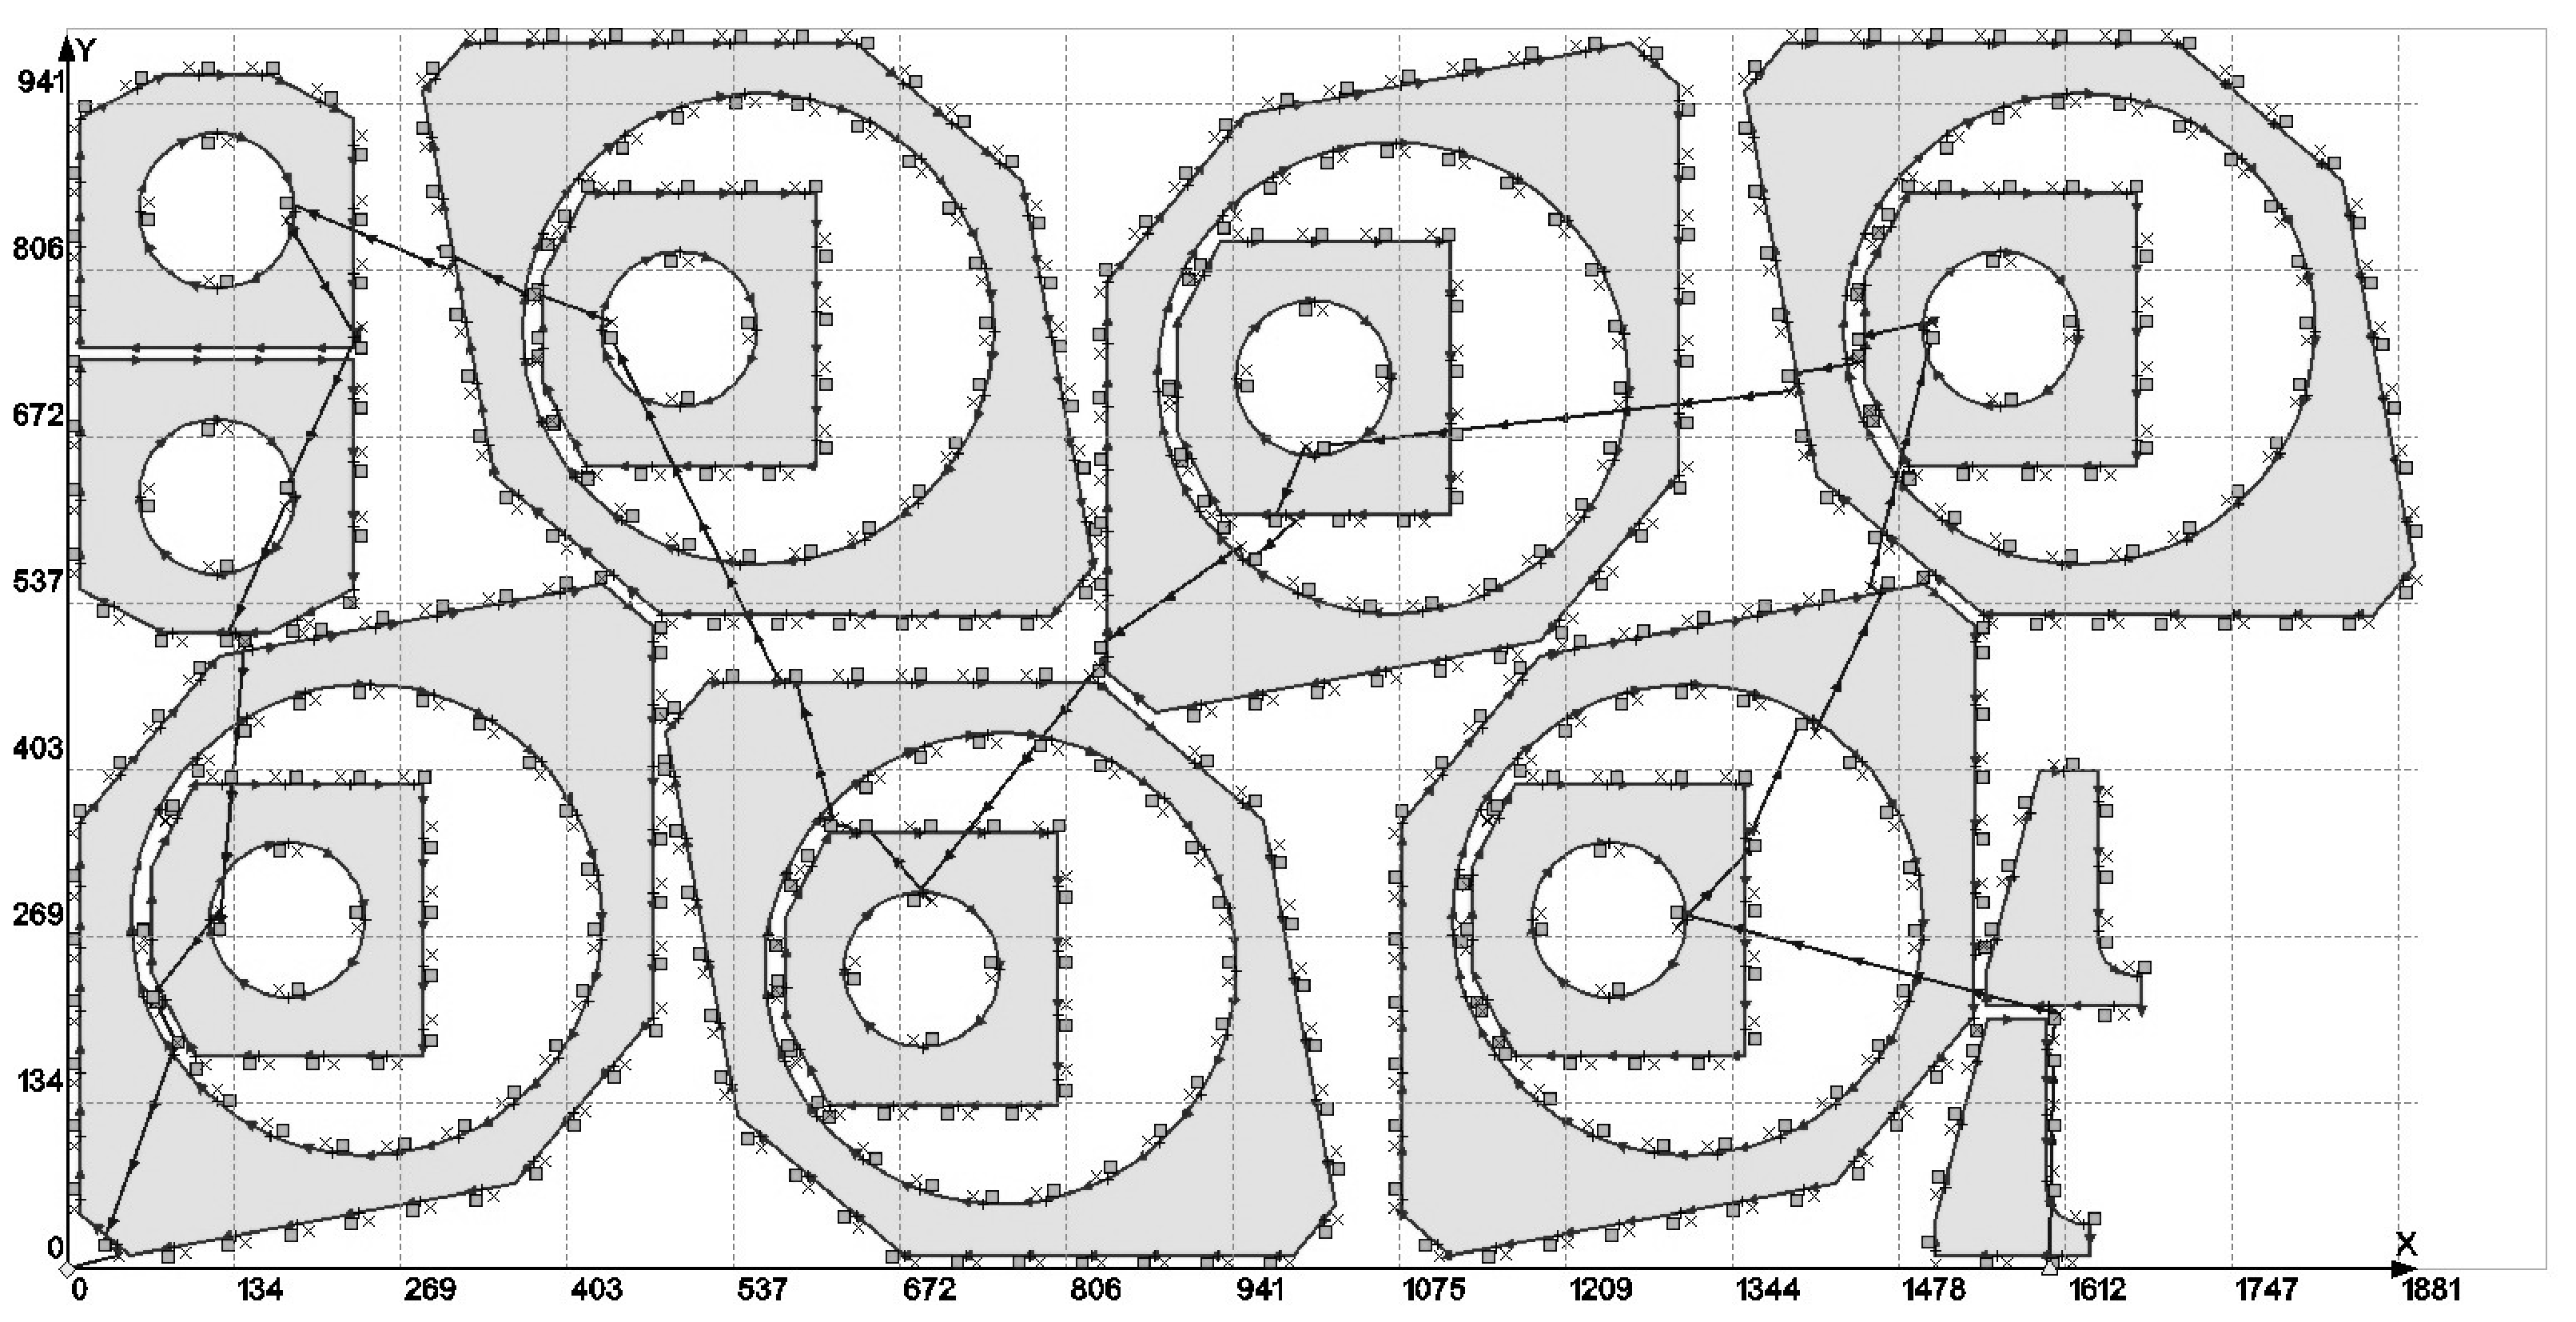
\includegraphics[width=120 mm]{image.pdf}
  \caption{The route and trajectory of set traversal}
  \label{fig:1}
\end{figure}

Figure~\ref{fig:2} shows another example of calculating the optimal tool path when cutting 18 parts defined by 24 contours. Possible pierce points are marked with green dots. The optimal starting point was not calculated in this example.
The extreme value of the objective function (total cutting time) was 2338 sec. Despite the decrease in the number of contours from 30 to 24, the time of finding the global extremum is also quite big (16 min 25 sec). This is because the number of precedence constraints in this example is less than in the first one.
The model of megalopolises is also applicable  when using non-standard cutting techniques,
in particular, the so-called ``multi-contour cutting'', which, as noted above, assumes the use of only
one pierce point for cutting two or more contours within one cutting segment.
Fig. \ref{fig:3} illustrates an example of calculating the optimal trajectory for the case of using the so-called "bridge" technique
(a special case of multi-contour cutting). The locations of the "bridges" connecting pairs of contours are indicated by black ovals, and the combined parts themselves are highlighted gray color. In this example, the time to search a global extremum was only 2 min 1 sec, since the number of megalopolises as a result of the unification of some of them decreased to 21. In this case, the total cutting time was 2323 sec. Adding one more bridge
(see Fig. \ref{fig:4}) reduces the time to obtain a global extremum by half (59 sec), while the value of the extremum (total time of the sheet cutting process ) is also slightly reduced (2318 sec). At the same time, all technological requirements for thermal cutting of parts on CNC sheet cutting machines are met.

These examples shows that the use of the model of megalopolises used as a discrete image of "base cutting segment",
allows searching optimal solutions for problems of the GSCCP class (Generalized Segment Continuous Cutting Problem) \cite{bibx:112}. In all cases, the objective function takes into account (as in the examples above) in addition to the parameters of the idle motion, also the the working cutting time and the total time for material piercing. These parameters are not constants due to changes in the number of megalopolises and the length of the working path of the tool. Instead of time parameters in the objective function, you can also use the cost parameters of cutting process \cite{Tavaeva}.

\begin{figure}
  \centering
  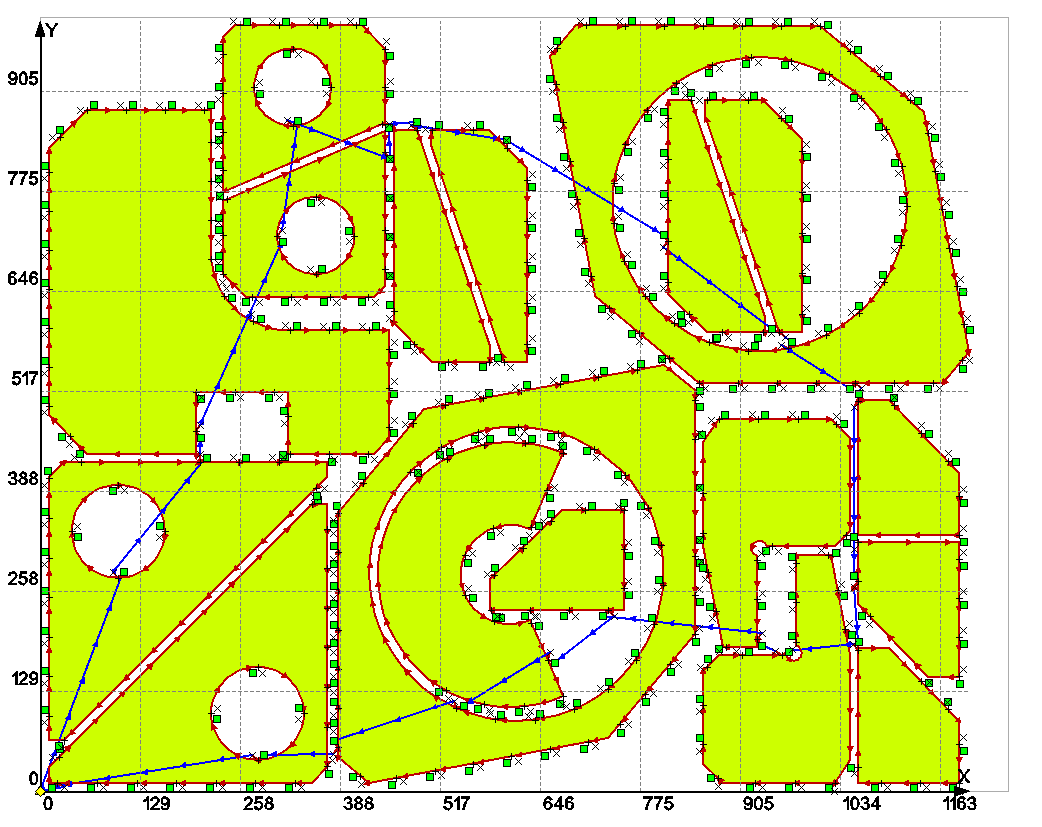
\includegraphics[width=120mm]{Fig2-18-24-green.png}
  \caption{Optimal cutting path for cutting of 24 contours when using the standard cutting technique}
  \label{fig:2}
\end{figure}

\begin{figure}
  \centering
  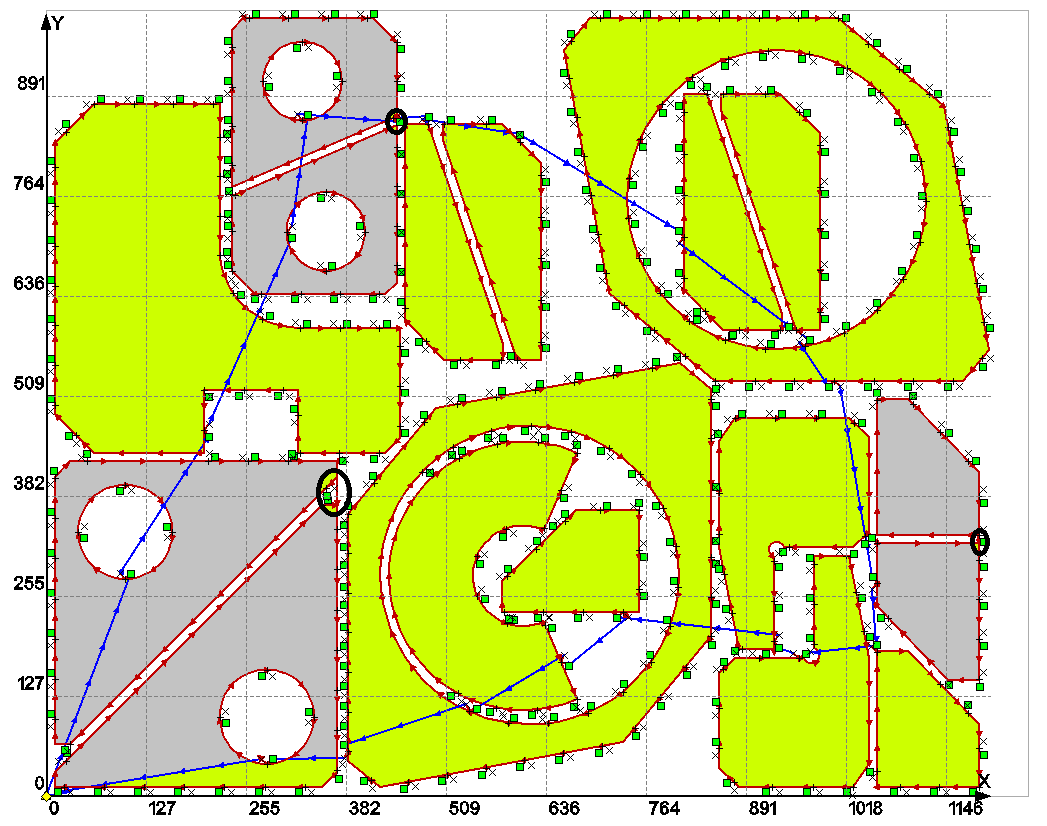
\includegraphics[width=120mm]{Fig3-21.png}
  \caption{Optimal cutting path when using the multi-contour cutting technique}
  \label{fig:3}
\end{figure}

\begin{figure}
  \centering
  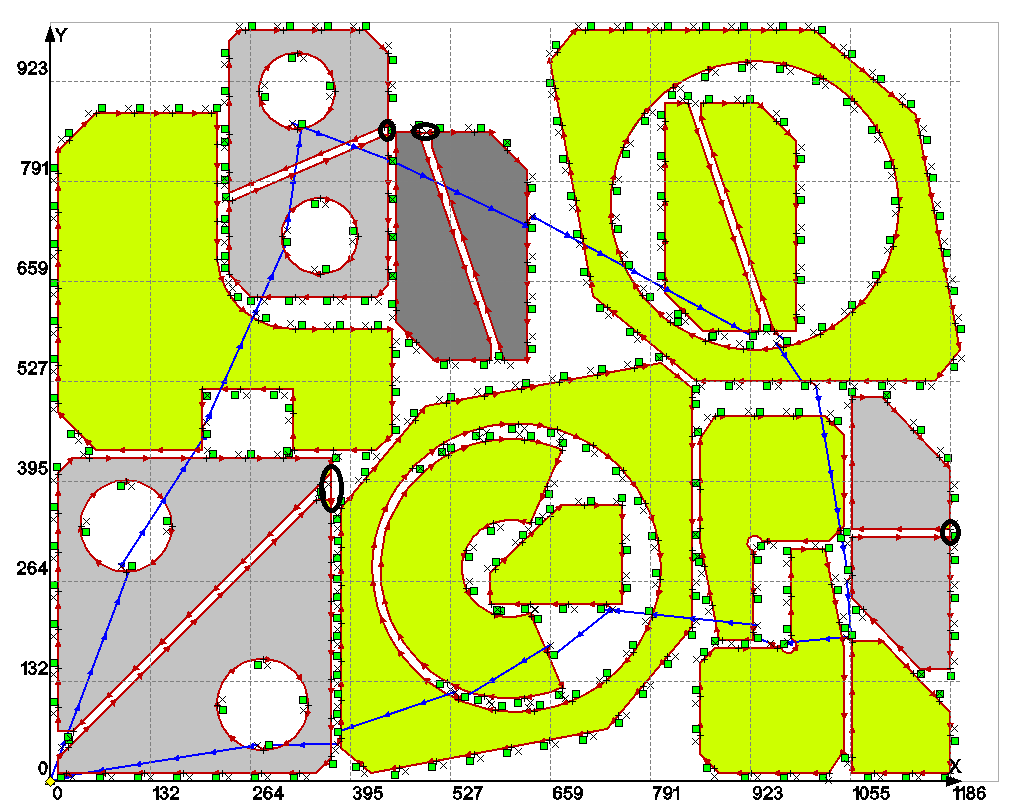
\includegraphics[width=120mm]{Fig4-20.png}
  \caption{Optimal cutting path obtained by developed algorithm in 1 min}
  \label{fig:4}
\end{figure}


It should be especially noted
that the mathematical model described in the chapter
makes it possible to obtain,
on an ordinary personal computer,
exact solutions for the tasks of tool path routing for CNC sheet-cutting machines for up to 30 or more (if we use non-standard cutting techniques) parts, while ensuring the manufacturability of the solution in terms of sheet cutting constraints based on heuristic rules (``a part hardness rule'' and ``a sheet hardness rule''). To comply with these rules, the routing algorithms described use the above-mentioned penalty mechanism. As noted above, the precedence constraints also significantly reduce the computational complexity of the problem.

Thus, summarizing the scientific aspects of the results obtained by the authors,
it can be emphasized that the proposed
theoretical constructions guarantee finding the global extremum of route optimization problems
in the range of problem sizes that are relevant for practice.
Further studies of the influence of the tool path on
the magnitude of thermal deformations of parts will ensure the compliance of the obtained exact solutions
to the real optimal and admissible technological routes for CNC sheet-cutting machines.

\sect{Conclusion\label{sec:6}}

The chapter explores routing problems focused on engineering applications associated with cutting of parts on CNC sheet cutting machines. At the same time, a very general formulation is presented that allows for other applications, among which we especially note the problem of successive dismantling of radiation on hazardous objects. For the aforementioned general arrangement of constructions, an optimal algorithm is based on a non-standard version of dynamic programming; the computational implementation of this algorithm is achieved for problems with a limited number of dimensions. In the general case, the scheme of the algorithm presented in the article determines the structure of the optimal solution, defined as a route process that includes the route itself (permutation of indices), the trajectory and the starting point. The entire mentioned complex (route process) is optimized under constraints including precedence conditions and cost functions depending on the list of tasks. These complications are motivated by the aforementioned engineering applications. Let's note the main stages of the research.

1. Formalization of the problem, including the model of metropolises, adequately taking into account the possible multivariance of the movements of the controlled object, and the strict definition of permissible routing processes. The precedence conditions are formulated and cost functions are introduced with a possible dependence on the list of tasks that have not been completed at a given time. Aggregation of costs is assumed to be additive.

2. Construction of an extension of the main problem to a system of partial problems, including a special reduction of precedence conditions (admissibility by precedence is equivalently replaced by admissibility by excluding tasks from the list). The Bellman equation, obtained in earlier works by the author, is used at the stage of constructing special layers of the Bellman function.

3. Implementation of an economical (through the use of precedence conditions) recurrent procedure, within which the construction of the entire array for the Bellman function values is replaced by the construction of its layers, which is essential from the point of view of reducing the computational complexity.

4. Searching of the global extremum and the optimal start point, for which a partial process is then constructed in the form of a route-trace pair, implemented in accordance with the previously constructed layers of the Bellman function. The result of the construction is the optimal route process that implements the global extremum and is obtained by adding the optimal starting point to the partial process of the previous stage.

5. In the problem of tool control during sheet cutting of parts on CNC machines, megalopolises in the simplest case are obtained by discretizing the equidistant contours to be cut (meaning cutting along a closed contour). However, other options for definitions metropolises are possible (and this is shown in the chapter), when it is allowed to combine several contours into one whole, or several fragments of contours, there are cutting segments in mind. With this approach, after some preliminary constructions in order to determine cost indicators, it turns out to be possible to reduce the dimension, which is essential in problems of this kind.

6. The prospect of solving large-scale problems can be associated, in particular, with the construction of optimizing inputs and multi-inputs, as well as iterative procedures using these inputs. In this case, of course, it is assumed that the optimizing inputs have a limited dimension, which allows for the use of dynamic programming in local versions (optimization in windows). It is also possible to use the branch and bound method and various metaheuristics.

%----------------------------------------------
\vspace{1ex}

\makeatletter
\@fundingeng\par
\@addtoreset{equation}{section}
\@addtoreset{footnote}{section}
\renewcommand{\section}{\@startsection{section}{1}{0pt}{1.3ex
plus 1ex minus 1ex}{1.3ex plus .1ex}{}}

\vspace{3ex}
\small
{ %\scriptsize

\renewcommand{\refname}{{\rm\centerline{REFERENCES}}}

% \bibliographystyle{abbrv}
\bibliographystyle{ieeetr}
\bibliography{Chentsov.bib}

\receivedeng

\contactseng

\titlerus

\pagestyle{basestylerus}

\referrus

\selectlanguage{russian}
\begin{center}
СПИСОК ЛИТЕРАТУРЫ
\end{center}
\setlength{\leftmargini}{1.8em}
\begin{enumerate}
\setlength{\itemsep}{0em}
\parskip=0pt

\item
V. V. Korobkin, A. N. Sesekin, O. L. Tashlykov, and A. G. Chentsov, Metody marshrutizatsii
i ikh prilozheniya v zadachakh povysheniya ehffektivnosti i bezopasnosti ehkspluatatsii atomnykh
stantsiy. Izdatel’stvo "Novye tekhnologii", 2012.

\end{enumerate}

\receivedrus

\contactsrus

\end{document}
